% !TEX root = ../main.tex


\section{Description of Sample Application}

To illustrate the development and analysis process of a design using the previously described 
statechart semantics, we will discuss a quadrotor helicopter or quadrotor application similar to 
the one presented by Syriani et al.~\cite{Syriani_2019}.The application will focus on the incremental 
design of some of the drone's required functionality.
The model constructed following statechart refinement rules that are proven within the Rodin tool.
The structure of the statechart for this model at each subsequent abstraction level restrict farther 
development of the model to refinements that obey the rules. This will allow us to prove properties 
of the model in a very strategic fashion, as properties proven of early abstraction levels 
are preserve in later refinements.

The first abstraction of the model shown in figure~\ref{fig:drone} captures the basic 
functionality of the drone. The model initial state is |OFF| and as a result of the |on| and 
|toTakeoff| external triggers it transitions to the |START| and |OPERATIONAL| respectively. 
The drone reacts to the |off| external trigger by shutting down and a subsequent transition to |OFF|.
Within the |OPERATIONAL| state the drone will transition to |FLY|, |DESCEND| or |LANDED| 
after the internal triggers |toFly|, |toLand| or |landed|. In this abstraction these interal 
triggers are raised non-deterministically in the system by functionality not currently defined.
As additional details are incoorporated into the model in later refinements some of that non-determinism is 
removed and replaced transitions with actions that raised the previously defined internal triggers.
\begin{figure}[!h]
	\vspace{-.4cm}
	\centering
	\includegraphics[width=0.99\textwidth]{figures/drone.png}
	\caption{Statechart of drone application. 1. Abstract level including only generic behavior 
	2. Refinement level introducing details for TakeOff 3. Refinement level for descending capabilities 
	4. Refinement level for battery consumption functionality. NOTE: this figure still needs a lot of work}
	\label{fig:drone}
	\vspace{-.4cm}
\end{figure} 
% \emph{Describe the Drone case study including refinements and things we would verify}
